In this section, we evaluate the effectiveness of our proposed methods for overcoming oscillations and compare them against other QAT methods on ImageNet \citep{imagenet}. We focus on low-bit quantization, 4 and 3 bits, of efficient networks with depth-wise separable convolutions, where the effect of weight oscillation is most pronounced. We start with our ablation studies, where we only quantize the weights in a network and, finally, present results for low-bit weight and activation quantization.

\subsection{Experimental setup}



\label{sec:experimentalconv.3.1_setup}

% \paragraph{Networks} We evaluate our methods using the \rn{18} \citep{resnet}, \mnv{2} \cite{mobilenetv2}, \mnv{3}-Small \citep{MobileNetV3} and EfficientNet-Lite \citep{EfficientNet}.

\paragraph{Quantization}
We follow the example of existing QAT literature and apply LSQ-type \citep{lsq} weight and activation quantization: we quantize all weights to a low bit-width while keeping the weights of the first and last layer to 8-bits, and quantize the input to all layers expect for the normalizing layers. We use per-tensor quantization \cite{krishnamoorthi} and learn the quantization scaling factor.

\paragraph{Optimization}
In all cases, we start from a pre-trained full-precision network and instantiate the weight and activation quantization parameters using MSE range estimation \citep{whitepaper}. We use SGD with a momentum of 0.9 and train using a cosine annealing learning-rate decay. We train for 20 epochs with only weight quantization for the ablation studies. For weight and activation quantization in section \ref{sec:comparison_to_qat_methods}, we train all models for 90 epochs. Depending on the network and quantization bit-width we train with a learning rate of either 0.01 or 0.0033. 


% we sweep through learning rates and present the results for the best one. 
% We train for 20 epochs using the Adam \cite{kingma2014adam} optimizer on both weights and quantization parameters and use a cosine annealing learning-rate decay (without restarts) $100\times$ than the initial learning rate. For each quantization regime, we sweep through learning rates and present the results for the best one. 

\subsection{Ablation studies}
\label{sec:ablation_studies}
\paragraph{Oscillation dampening}
In table \ref{tbl:ocillation_dampening_ablation} we study how the strength of the dampening loss affects the network's final accuracy and the proportion of oscillating weights at the end of training. In the first three rows, we observe that as we increase the coefficient $\lambda$, the proportion of oscillating weights decreases and the gap between pre and post-BN re-estimation accuracy closes. However, too much dampening harms the final accuracy, suggesting that excessive regularization inhibits beneficial movement of weights between quantization levels.

Our solution to this problem is to gradually increase the regularization strength during training. This allows the latent weights to move more freely in the first stages of training, while reducing harmful oscillations close to convergence by applying a stronger regularization. We find that a cosine annealing schedule for $\lambda$ works well in practice. \citet{binreg} also notice that such a regularization is harmful at the early stages of training but instead adopt a two-stage optimization process. We see that such a strategy can significantly dampen the oscillations while not harming the accuracy. The best damping configuration improves almost 1\% over the post-BN re-estimation baseline and more than 5\% over the pre-BN re-estimation baseline.

In figure \ref{fig:bin_distribution_freezing_damp} (left), we also visualize the effect of dampening on the latent weight distribution of the same depth-wise separable layer as in figure \ref{fig:mv2_bin_distribution}. As intended, the latent weights are now clustered around the quantization bin centres with hardly any weights at the decision boundary. 

\begin{table}[t]
    \centering
    \begin{tabular}{ l | c  c  c }
    \toprule
    %   &     \multicolumn{2}{c|}{Accuracy} &  \\
  Regulatization & pre-BN &  post-BN & Osc.(\%) \\
        \midrule
Baseline  & 64.97\textsuperscript{1.23} & 69.50\textsuperscript{0.04} & 4.93\\
\midrule
$\lambda=10^{-4}$   & 65.97\textsuperscript{1.52}       &  69.65\textsuperscript{0.08} &  2.18 \\
$\lambda=10^{-3}$   & {66.99}\textsuperscript{1.41}     & \textbf{69.96}\textsuperscript{0.12} & 0.21 \\
$\lambda=10^{-2}$	& \textbf{68.04}\textsuperscript{1.04}  & 68.57\textsuperscript{0.07} & 0.01 \\
\midrule
% cosine $\lambda=[0, 10]$  & 69.47 & 55.79 &\\ 
% cosine $\lambda=[0, 1e3]$  & \textbf{69.91}\textsuperscript{0.06} & 68.34\textsuperscript{1.31} &\\ 
% cosine $\lambda=[0, 1e4]$  & \textbf{69.80}\textsuperscript{0.15} & 69.63\textsuperscript{0.18} &\\ 
$\lambda=\cos(0, 10^{-4})$  & 64.47\textsuperscript{1.59} & 69.61\textsuperscript{0.07} & 2.64 \\ 
$\lambda=\cos(0, 10^{-3})$  & {68.79}\textsuperscript{1.31} & \textbf{70.37}\textsuperscript{0.06} & 1.63 \\ 
$\lambda=\cos(0, 10^{-2})$  & \textbf{70.18}\textsuperscript{0.18} & 70.26\textsuperscript{0.08} & 1.11 \\ 
\bottomrule
\end{tabular}
 \caption{Effect of oscillation dampening strength and schedule in the final accuracy of \mnv{2} with 3-bit weight quantization. \textit{post-BN}: accuracy after BN re-estimation, \textit{pre-BN}: accuracy before BN re-estimation. \textit{Osc.}: percentage of oscillating weights at the end of training ($f>0.005$). We report the average of 3 seeds and the STD in the superscript.}
 \label{tbl:ocillation_dampening_ablation}
\end{table}

\begin{table}[t]
    \centering
    \begin{tabular}{ l | c  c c }
    \toprule
    %   &     \multicolumn{2}{c|}{Accuracy} &  \\
  Method &   pre-BN & post-BN & Osc.(\%)\\
        \midrule
Baseline & 64.97\textsuperscript{1.23} & 69.50\textsuperscript{0.04} &  4.93 \\
\midrule
$f_{\text{th}}$= 0.02 & 68.13\textsuperscript{2.14}  & 69.96\textsuperscript{0.04} &   2.93 \\
$f_{\text{th}}$= 0.015 & \textbf{69.79}\textsuperscript{0.07} & \textbf{70.13}\textsuperscript{0.05} &  1.23\\
$f_{\text{th}}$= 0.01  &  69.12\textsuperscript{0.53} & 69.18\textsuperscript{0.47}  &   0.06 \\
\midrule
$f_{\text{th}}$= cos(0.04,0.015)  &  69.51\textsuperscript{0.15}  & 69.96\textsuperscript{0.03} &  2.33 \\
$f_{\text{th}}$= cos(0.04,0.01)  &  \textbf{69.97}\textsuperscript{0.06}  & \textbf{70.33}\textsuperscript{0.07} &  0.04 \\
% $f_{\text{th}}=\cos{(0.04,0.01)}$  &  xx\textsuperscript{x.xx}  & xx\textsuperscript{x.xx} &  xx\% \\
\bottomrule
\end{tabular}
 \caption{Effect of oscillation frequency threshold ($f_{\text{th}}$) on training of \mnv{2} with 3-bit weight quantization. \textit{post-BN}: accuracy after BN re-estimation, \textit{pre-BN}: accuracy before BN re-estimation, \textit{Osc.}: percentage of oscillating weights at the end of training ($f>0.005$). We report the average of 3 seeds and the STD in the superscript.}
 \label{tbl:weight_freezing_ablation}
\end{table}



% \begin{table}[h]
%     \centering
%     \begin{tabular}{ l | c  c c c }
%     \toprule
%     %   &     \multicolumn{2}{c|}{Accuracy} &  \\
%   $f_{\text{th}}$ &   pre-BN & post-BN &$ \delta$ & frozen\\
%         \midrule
% Baseline & & & & \\
% \midrule
% 0.04 &67.85\textsuperscript{0.22} &  69.57\textsuperscript{0.04} & +1.72 & xx\%\\
% 0.02 & \textbf{69.73}\textsuperscript{0.08}  &  \textbf{69.97}\textsuperscript{0.04} &  +0.24 & xx\%\\
% 0.015 & 69.18\textsuperscript{0.53} & 69.29\textsuperscript{0.47} &  +0.11 & xx\%\\
% 0.01  &  67.07\textsuperscript{0.00} & 67.14\textsuperscript{0.00}  &  +0.07 & xx\%\\
% \midrule
% $\cos\text{(0.1, 0.01)}$  &  xx\textsuperscript{x.xx}  & xx\textsuperscript{x.xx} &  +x.xx & xx\%\\
% \bottomrule
% \end{tabular}
%  \caption{Effect of oscillation frequency threshold ($f_{\text{th}}$) on training of \mnv{2} with 3-bit weight quantization. \textit{post-BN}: accuracy after batch-norm statistics re-estimation, \textit{pre-BN}: accuracy before batch-norm statistics re-estimation, $\delta$: difference between post-BN and pre-BN accuracy. We present the average of 3 seeds and the STD in the superscript }
%  \label{tbl:weight_freezing_ablation}
% \end{table}


% \begin{table}[h]
%     \centering
%     \begin{tabular}{ l | c  c  c }
%     \toprule
%     %   &     \multicolumn{2}{c|}{Accuracy} &  \\
%   $f_{\text{th}}$ &   pre-BN & post-BN & frozen\\
%         \midrule
% Baseline & & & \\
% \midrule
% 0.04 &67.85\textsuperscript{0.22} &  69.57\textsuperscript{0.04} &  xx\%\\
% 0.02 & \textbf{69.73}\textsuperscript{0.08}  &  \textbf{69.97}\textsuperscript{0.04} & xx\%\\
% 0.015 & 69.18\textsuperscript{0.53} & 69.29\textsuperscript{0.47} &  xx\%\\
% 0.01  &  67.07\textsuperscript{0.00} & 67.14\textsuperscript{0.00}  &  xx\%\\
% \midrule
% $\cos\text{(0.1, 0.01)}$  &  xx\textsuperscript{x.xx}  & xx\textsuperscript{x.xx} &  xx\%\\
% \bottomrule
% \end{tabular}
%  \caption{Effect of oscillation frequency threshold ($f_{\text{th}}$) on training of \mnv{2} with 3-bit weight quantization. \textit{post-BN}: accuracy after batch-norm statistics re-estimation, \textit{pre-BN}: accuracy before batch-norm statistics re-estimation, $\delta$: difference between post-BN and pre-BN accuracy. We present the average of 3 seeds and the STD in the superscript }
%  \label{tbl:weight_freezing_ablation}
% \end{table}


\begin{figure}[t]
\centering
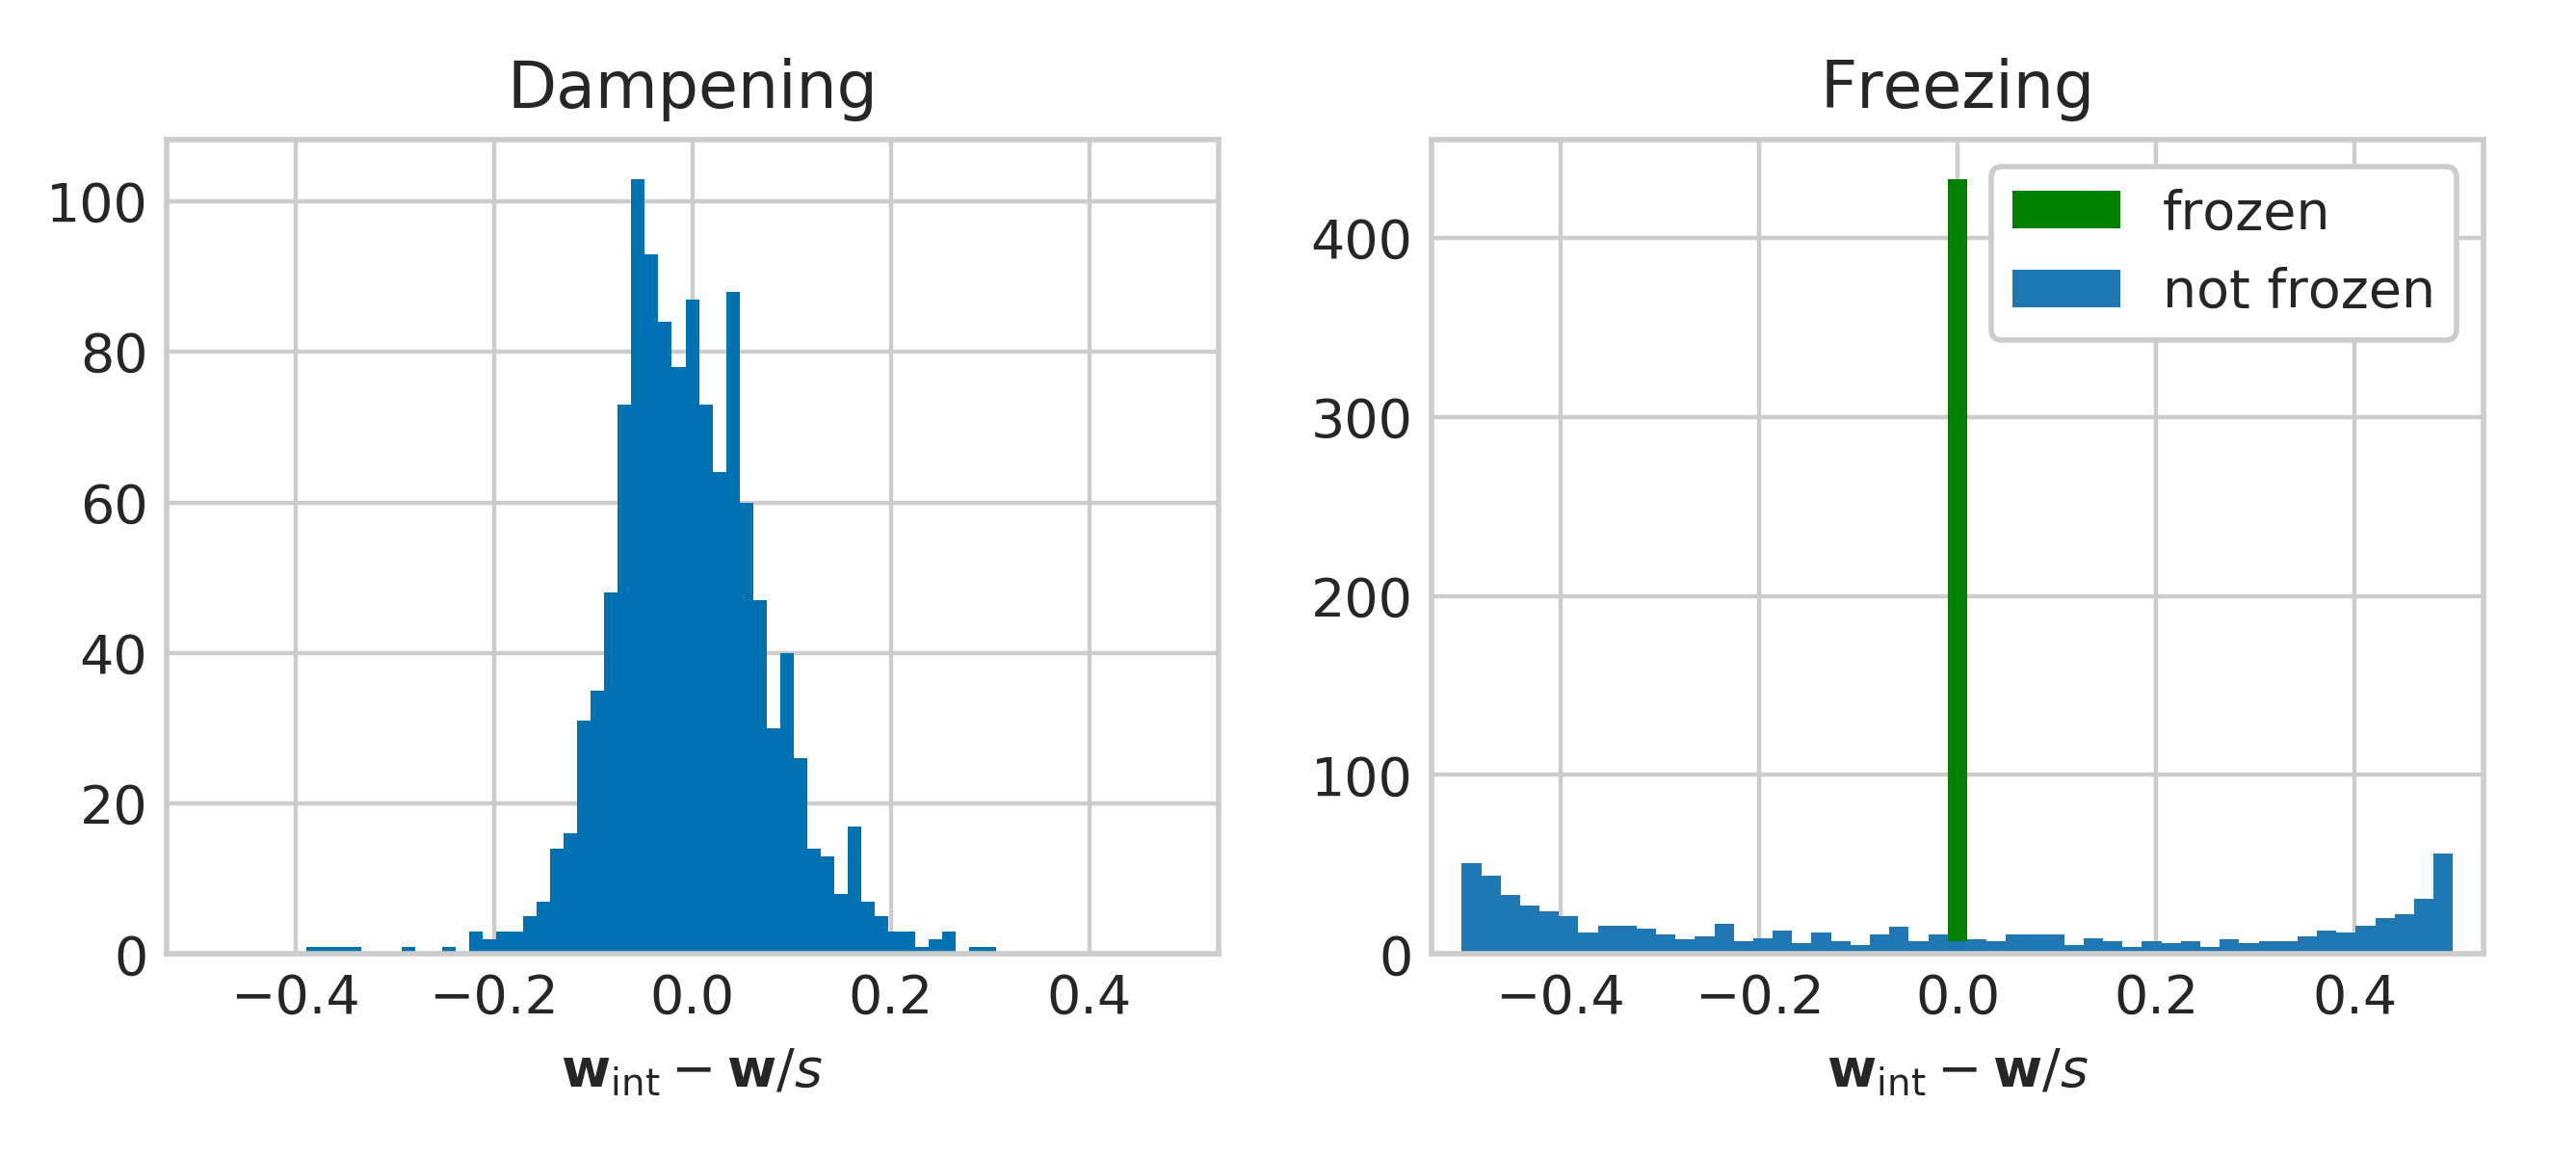
\includegraphics[width=1.\linewidth]{figures/mnv2_bin_dist_lsq_binReg_freeze_v2.png} 
\vspace{-0.8cm}
\caption{ Histogram of the distance of latent weights of layer conv.3.1 of \mnv{2} from their closest quantization grid-point after training with oscillation dampening (left) or iterative weight freezing (right).} 
\vspace{-0.1cm}
\label{fig:bin_distribution_freezing_damp}
\end{figure}


\paragraph{Iterative weight freezing}
% \begin{table}[t]
    \centering
    \begin{tabular}{ l | c  c c }
    \toprule
    %   &     \multicolumn{2}{c|}{Accuracy} &  \\
  Method &   pre-BN & post-BN & Osc.(\%)\\
        \midrule
Baseline & 64.97\textsuperscript{1.23} & 69.50\textsuperscript{0.04} &  4.93 \\
\midrule
$f_{\text{th}}$= 0.02 & 68.13\textsuperscript{2.14}  & 69.96\textsuperscript{0.04} &   2.93 \\
$f_{\text{th}}$= 0.015 & \textbf{69.79}\textsuperscript{0.07} & \textbf{70.13}\textsuperscript{0.05} &  1.23\\
$f_{\text{th}}$= 0.01  &  69.12\textsuperscript{0.53} & 69.18\textsuperscript{0.47}  &   0.06 \\
\midrule
$f_{\text{th}}$= cos(0.04,0.015)  &  69.51\textsuperscript{0.15}  & 69.96\textsuperscript{0.03} &  2.33 \\
$f_{\text{th}}$= cos(0.04,0.01)  &  \textbf{69.97}\textsuperscript{0.06}  & \textbf{70.33}\textsuperscript{0.07} &  0.04 \\
% $f_{\text{th}}=\cos{(0.04,0.01)}$  &  xx\textsuperscript{x.xx}  & xx\textsuperscript{x.xx} &  xx\% \\
\bottomrule
\end{tabular}
 \caption{Effect of oscillation frequency threshold ($f_{\text{th}}$) on training of \mnv{2} with 3-bit weight quantization. \textit{post-BN}: accuracy after BN re-estimation, \textit{pre-BN}: accuracy before BN re-estimation, \textit{Osc.}: percentage of oscillating weights at the end of training ($f>0.005$). We report the average of 3 seeds and the STD in the superscript.}
 \label{tbl:weight_freezing_ablation}
\end{table}



% \begin{table}[h]
%     \centering
%     \begin{tabular}{ l | c  c c c }
%     \toprule
%     %   &     \multicolumn{2}{c|}{Accuracy} &  \\
%   $f_{\text{th}}$ &   pre-BN & post-BN &$ \delta$ & frozen\\
%         \midrule
% Baseline & & & & \\
% \midrule
% 0.04 &67.85\textsuperscript{0.22} &  69.57\textsuperscript{0.04} & +1.72 & xx\%\\
% 0.02 & \textbf{69.73}\textsuperscript{0.08}  &  \textbf{69.97}\textsuperscript{0.04} &  +0.24 & xx\%\\
% 0.015 & 69.18\textsuperscript{0.53} & 69.29\textsuperscript{0.47} &  +0.11 & xx\%\\
% 0.01  &  67.07\textsuperscript{0.00} & 67.14\textsuperscript{0.00}  &  +0.07 & xx\%\\
% \midrule
% $\cos\text{(0.1, 0.01)}$  &  xx\textsuperscript{x.xx}  & xx\textsuperscript{x.xx} &  +x.xx & xx\%\\
% \bottomrule
% \end{tabular}
%  \caption{Effect of oscillation frequency threshold ($f_{\text{th}}$) on training of \mnv{2} with 3-bit weight quantization. \textit{post-BN}: accuracy after batch-norm statistics re-estimation, \textit{pre-BN}: accuracy before batch-norm statistics re-estimation, $\delta$: difference between post-BN and pre-BN accuracy. We present the average of 3 seeds and the STD in the superscript }
%  \label{tbl:weight_freezing_ablation}
% \end{table}


% \begin{table}[h]
%     \centering
%     \begin{tabular}{ l | c  c  c }
%     \toprule
%     %   &     \multicolumn{2}{c|}{Accuracy} &  \\
%   $f_{\text{th}}$ &   pre-BN & post-BN & frozen\\
%         \midrule
% Baseline & & & \\
% \midrule
% 0.04 &67.85\textsuperscript{0.22} &  69.57\textsuperscript{0.04} &  xx\%\\
% 0.02 & \textbf{69.73}\textsuperscript{0.08}  &  \textbf{69.97}\textsuperscript{0.04} & xx\%\\
% 0.015 & 69.18\textsuperscript{0.53} & 69.29\textsuperscript{0.47} &  xx\%\\
% 0.01  &  67.07\textsuperscript{0.00} & 67.14\textsuperscript{0.00}  &  xx\%\\
% \midrule
% $\cos\text{(0.1, 0.01)}$  &  xx\textsuperscript{x.xx}  & xx\textsuperscript{x.xx} &  xx\%\\
% \bottomrule
% \end{tabular}
%  \caption{Effect of oscillation frequency threshold ($f_{\text{th}}$) on training of \mnv{2} with 3-bit weight quantization. \textit{post-BN}: accuracy after batch-norm statistics re-estimation, \textit{pre-BN}: accuracy before batch-norm statistics re-estimation, $\delta$: difference between post-BN and pre-BN accuracy. We present the average of 3 seeds and the STD in the superscript }
%  \label{tbl:weight_freezing_ablation}
% \end{table}

In table \ref{tbl:weight_freezing_ablation}, we demonstrate the effectiveness of our iterative weight freezing algorithm for various freezing thresholds. Using a constant threshold throughout training, we see that the amount of remaining oscillations significantly reduces with a decreasing threshold and only some low frequency oscillations remain in the network. We also see that the pre-BN re-estimation accuracy is  closer to the the post-BN re-estimation accuracy, as one would expect when there are fewer oscillations at the end of training. 

\begin{table}[t]
    \centering
    \begin{tabular}{ l | c |  c }
    \toprule

  Method & W/A &    Val. Acc. (\%)  \\
        \midrule
Full-precision & 32/32 & 71.7 \\
\midrule
LSQ* \citep{lsq}         & 4/4 & 69.5 (-2.3) \\ %71.8
PACT \cite{pact2018}    & 4/4 & 61.4  (-10.3)\\ % Assume 71.8
DSQ \citep{DSQ}         & 4/4 & 64.8 (-6.9) \\
EWGS \citep{EWGS}       & 4/4 & 70.3 (-1.6) \\ % 71.9
% PROFIT \citep{profit}   & 4/4 & 71.6 \\
LSQ + BR \citep{binreg} & 4/4 & 70.4 (-1.4)\\ %71.8
LSQ + Dampen (ours)     & 4/4 & \textbf{70.5} (-1.2) \\
LSQ + Freeze (ours)     & 4/4 & \textbf{70.6} (-1.1) \\
\midrule
LSQ* \citep{lsq}         & 3/3 & 65.3 (-6.5)  \\
LSQ + BR \citep{binreg} & 3/3 & 67.4 (-4.4) \\
LSQ + Dampen (ours)     & 3/3 & \textbf{67.8} (-3.9)  \\
LSQ + Freeze (ours)     & 3/3 & \textbf{67.6} (-4.1) \\
\bottomrule
\end{tabular}
 \caption{Comparison of oscillation dampening and freezing with other QAT methods for \mnv{2} on ImageNet classification. We report validation accuracy (\%) and the difference to the corresponding full precision baseline. Note, both \citet{binreg} and \citet{EWGS} use a slightly higher baseline model. *results from \citet{binreg}.}
 \vspace{-0.1cm}
 \label{tbl:final_results_mnv2}
\end{table}


\begin{table}[t]
    \centering
    \begin{tabular}{ l | c |  c }
    \toprule

  Method & W/A &    Val. Acc. (\%)  \\
        \midrule
Full-precision & 32/32 & 65.1 \\
\midrule
LSQ* \citep{lsq}         & 4/4 & 61.0  \\
LSQ + BR \citep{binreg} & 4/4 & 61.5 \\
LSQ + Dampen (ours)     & 4/4 & \textbf{63.7}  \\ 
LSQ + Freeze (ours)     & 4/4 &  \textbf{63.6} \\
\midrule
LSQ* \citep{lsq}         & 3/3 &  52.0 \\
LSQ + BR \citep{binreg} & 3/3 &   56.0 \\
LSQ + Dampen (ours)     & 3/3 &   \textbf{59.0}  \\
LSQ + Freeze (ours)     & 3/3 &   \textbf{58.9} \\
\bottomrule
\end{tabular}
 \caption{Comparison of oscillation dampening and freezing with other QAT methods for \mnv{3}-Small on ImageNet classification. We report validation accuracy (\%). *results from \citet{binreg}.}
 \label{tbl:final_results_mnv3}
\end{table}


\begin{table}[t]
    \centering
    \begin{tabular}{ l | c |  c }
    \toprule

  Method & W/A &    Val. Acc. (\%)  \\
        \midrule
Full-precision          & 32/32 & 75.4 \\
\midrule
LSQ* \citep{lsq}         & 4/4 &  72.3 \\
LSQ + Dampen (ours)     & 4/4 &  \textbf{73.5} \\
LSQ + Freeze (ours)     & 4/4 &  \textbf{73.5} \\
\midrule
LSQ* \citep{lsq}         & 3/3 &  69.7 \\
LSQ + Dampen (ours)     & 3/3 &  \textbf{71.1}  \\
LSQ + Freeze (ours)     & 3/3 &  \textbf{71.0} \\
\bottomrule
\end{tabular}
 \caption{Comparison of oscillation dampening and freezing for EfficientNet-lite on ImageNet classification. We report validation accuracy (\%). *our re-implementation.}
 \label{tbl:final_results_en_lite}
\end{table}


% \begin{table*}[t]
%     \centering
%     \begin{tabular}{ l | c |   c  c  c}
%     \toprule

%   Method & W/A &    \mnv{2} &  \mnv{3}-Small& EfficientNet-lite \\
%         \midrule
% Full-precision & 32/32 & 71.72 & 65.1 & 75.42 \\
% \midrule
% LSQ \citep{lsq}       & 4/4 & 69.5+ &  - & 72.34* \\
% PACT \cite{pact2018}  & 4/4 & 61.4 &  - & -\\
% DSQ \citep{DSQ}      & 4/4 & 64.8 &  - & -  \\
% EWGS \citep{EWGS}    & 4/4 & 70.3 & - & - \\
% PROFIT \citep{profit}  & 4/4 & 71.6 & - & - \\
% LSQ + BR \citep{binreg} & 4/4 & 70.4 & - & - \\
% LSQ + Dampen (ours) & 4/4 &   & - & - \\
% LSQ + Freeze (ours)  & 4/4 &   & - & 73.48 \\
% \midrule
% LSQ \citep{lsq}       & 3/3 & 65.3+ &  - & 69.72* \\
% LSQ + BR \citep{binreg}  & 3/3 & 67.4 & - & - \\
% LSQ + Dampen (ours)  & 3/3 &   & - & - \\
% LSQ + Freeze (ours)  & 3/3 &   & - & 70.94 \\
% \bottomrule
% \end{tabular}
%  \caption{Comparison of method with other QAT methods on ImageNet classification. We report average top-1 validation accuracy over 3 seeds. +results from \citet{binreg}, *our implementation}
%  \label{tbl:final_results}
% \end{table*}



However, we note that if the oscillation threshold becomes too low, too many weights get frozen in the early stages of training reducing the final accuracy. To address this, we apply an annealing schedule to the freezing threshold similar to the one used in dampening. This allows us to use a stronger freezing threshold and freeze almost all oscillations towards the end of training, when they are most disruptive.  The best freezing threshold improves almost 1\% over the post BN re-estimation baseline and more than 5\% over the pre BN re-estimation baseline. Its accuracy is on par with the oscillation dampening while having significantly less remaining oscillations (0.04\% vs 1.11\%).

In figure \ref{fig:bin_distribution_freezing_damp} (right), we see how iterative weight freezing changes the latent weight distribution of layer conv.3.1 of \mnv{2}. The majority of the latent weights are now frozen at the bin centres removing the peaks observed at the decision boundary in figure \ref{fig:mv2_bin_distribution}.


% shows the final latent latent weight distribution for the depth-wise separable

% In figure \ref{fig:bin_distribution_freezing_damp} (right) we visualize how freezing affects the final latent weight distribution for the depth-wise separable convolution conv.3.1 of \mnv{2}. The distribution peaks at the quantization boundaries anymore from figure \ref{fig:mv2_bin_distribution} (right) are now gone as these weight have now been frozen to the quantization bin centre.

\subsection{Comparison to other QAT methods}
\label{sec:comparison_to_qat_methods}
We compare our methods for overcoming oscillation  to other QAT alternatives and demonstrate their effectiveness in low-bit quantization of popular efficient neural networks. To compare to existing methods in the literature we quantize both weights and activations. 
In table \ref{tbl:final_results_mnv2}, we show the results for \mnv{2} and demonstrate that both our algorithms outperform all competing QAT techniques in literature for 3 and 4-bit quantization. We also achieve state-of-the-art results for \mnv{3}-Small and \efnet{lite} in tables \ref{tbl:final_results_mnv3} and \ref{tbl:final_results_en_lite}, respectively. In all cases, our oscillation prevention methods significantly improve ($>1\%$) over the commonly used LSQ baseline, showing the general applicability of our methods to other efficient networks.

We note that oscillation dampening leads to an increase of approximately 33\% in training time compared to the LSQ baseline. A similar trend was also observed by \cite{binreg}. On the other hand, iterative weight freezing has a negligible computational overhead while achieving similar performance.
